\section{Background}
\subsection{Unreliable Communication in Numerical Programs}
In recent years, various approximation techniques that allow
computations to continue in the face errors have become popular.
A lot of work has looked into handling synchronization errors and
other types of communication errors. 

Various networking techniques have been proposed that can drop
messages to free up contested network resources in order to speed up
communication. Our experiments with such a proposed network on chip
architecture have shown that many numerical programs (from popular
benchmark suites such as Parsec) can produce acceptable results in the
face of many messages among being dropped. In extremely unreliable
settings where up to 20\% of messages were dropped, we observed results
that were $<1\%$ different to the baseline.
For example, 
\begin{itemize}
  \item Volrend (Parsec) - Renders a 3D object.
Can drop 30\% messages related to some data structures while keeping
the PSNR of the generated image at 37.2 dB
\item Connected Components - Computes connected components of a graph.
Can drop 20\% messages while keeping the fraction of erroneous nodes under 0.0007
\item Bodytrack (Parsec) - Tracks a body pose through a set of images.
Can drop 11\% of messages while keeping the average relative difference
of poses under 0.09
\end{itemize}


\subsection{Statistical Model Checking}
Model checking is a powerful technique to automatically verify properties of a system. First a model is defined and a set of properties that need to be verified are specified. Model checking systematically explores the state space of the model to check if there is any path in the model which violates the properties. Standard model checking can find paths that violate the properties but it doesn't provide any information about the importance pf the path in which violation is found. Statistical model checking seeks to address this weakness by augmenting the violations found in the model with probability of the violation. With this information, a developer can focus on the most probable bugs first.

Statistical model checking requires a model which contains information about the probabilities of transition. Statistical model checkers simulate the system considering the probabilities of different transitions. This simulation gives a sample path. The properties that need to be check are tested on this sample path. The properties are either satisfied or violated giving a boolean outcome. A large number of simulations are performed and probability of a property violation is estimated as (number of violations / number of samples). the number of samples is also used to estimate a confidence interval for the probabilities. Statistical model checking also enables checking properties that define probabilistic bounds on a system. An example of such a property for a server processing jobs from a bounded queue is that the probability that the queue is full is less than 1\% (in other words system availability is greater than 99\%). The properties for statistical model checking are commonly specified in Probabilistic Computation Tree Logic (PCTL). This is a probabilistic extension of Computation Tree Logic (CTL) and allows including probability bounds in the property specifications.

In this project we are using PRISM model checker. PRISM allows us to specify probabilistic models as DTMC's which we are using for modeling IOT systems. We identify unacceptable states based on the logic of the IOT system being modeled. PRISM can also calculate analytical results for small models which can be used instead of sampling based statistical model checking for small models.

\subsection{IOT System Models}

\begin{figure} 
  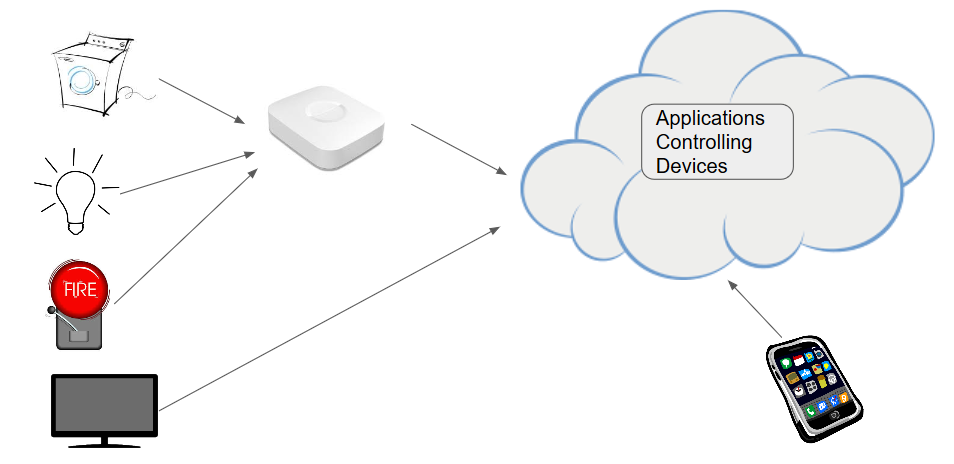
\includegraphics[width=\textwidth]{IOT.PNG}
  \caption{General Architecture of IOT Systems}
  \label{IOT}
\end{figure}

Figure \ref{IOT} shows the general architecture of IOT systems. Most smart devices which support remote monitoring and control do not have enough resources to support full Internet connectivity. These are called constrained resource devices and support some Personal Area Network (PAN) protocol like Zigbee or Bluetooth. While it is possible to manufacture devices that connect directly to Internet, managing all the risks that come with such a connection can increase the cost of the device. Different manufacturers have released devices called hubs which support several Personal Area Network (PAN) protocols to connect with devices and also connect with Internet. These hubs are responsible for providing safe access to the devices connected to the hub through the Internet. While most simple devices connect with the Internet through the hub, there are devices which can connect directly with the Internet. These devices are normally high end devices like smart TV's which need to have Internet access to provide entertainment services to the users.

The cloud back-end in IOT systems is the glue that holds the complete system together. It can notify the user about the status of the devices and it enables the devices to interact with each other as well. For example: A smart thermostat detects that a room is getting too hot and air conditioner needs to be turned on. But before turning on the air conditioner, the thermostat notifies the cloud back-end. Cloud back-end checks the sensors in the rooms and determines that the room is empty so there is not need to turn on the air conditioner. These rules which are enforced by the cloud are sometime called IOT applications. These applications can also make use of external sources of information like weather data, time and date, user's social media accounts and alerting emergency services on behalf of the user.

Since all components of an IOT system connect to the cloud, it is possible, in theory, that any device can talk to any other device in the system. In practice, we observe that an IOT system can usually be broken down into several subsystems. For example, one subsystem consisting of multiple devices may be dedicated to intrusion detection. This subsystem is should not be concerned with the status of the laundry. This separation into independent subsystems become clear when we look into the functionality of the applications deployed in the cloud. This gives us an opportunity of reducing the size of the system we need to model to check for various properties. We use this property when we present a model for the security subsystem of a house later in this report.
